\documentclass{article}
\usepackage[main,final]{neurips_2026}
\makeatletter
\renewcommand{\@noticestring}{}
\makeatother
\usepackage[utf8]{inputenc}
\usepackage[T1]{fontenc}
\usepackage{hyperref}
\usepackage{url}
\usepackage{booktabs}
\usepackage{amsmath}
\usepackage{amsfonts}
\usepackage{graphicx}
\usepackage{microtype}
\usepackage{xcolor}
\usepackage{float}
\usepackage{caption}
\captionsetup{font=small,skip=3pt}
\setcounter{topnumber}{4}\setcounter{totalnumber}{6}\renewcommand{\topfraction}{0.9}\setlength{\textfloatsep}{8pt plus 2pt minus 2pt}
\setlength{\floatsep}{6pt plus 2pt minus 2pt}
\setlength{\intextsep}{6pt plus 2pt minus 2pt}

\title{Search over Reasoning: A Prompted Step Verifier\\versus Repeated Sampling on GSM8K}
\author{Daniyal Hussain Shah\\Roll No.\ 28100434\\15 November 2026}

\begin{document}
\maketitle

\begin{abstract}
Test-time search can improve a fixed language model, but a step-level verifier adds many model calls. This report asks whether such a verifier beats plain repeated sampling on 50 GSM8K problems. A Qwen2.5-1.5B-Instruct generator writes five shared candidate solutions per problem, and a 4-bit Qwen2.5-7B-Instruct judge labels every step as valid or invalid. Best-of-five selection by path score reaches 70.0\%, against 56.0\% for greedy decoding and 64.0\% for five-sample self-consistency (SC), but 15-sample SC reaches 80.0\% with fewer calls. With 50 problems, none of the gaps between verified search and sampling is statistically established. Min-pooling, product, and step-penalty scores give identical accuracy, because the judge mainly filters out paths that contain an invalid step. In a hand audit of 40 steps the judge has 45\% precision and 82\% recall for invalid steps, and 25\% of incorrect paths pass every step. Under a budget of ten times the greedy output tokens, self-consistency is the better use of compute. Code and results are available at \url{https://github.com/syeddaniyalg/cs5326-pa3}.
\end{abstract}

\section{Introduction}
Extra computation at inference time can improve a fixed model. The simplest form samples several solutions and takes a majority vote \citep{wang2023selfconsistency,brown2024monkeys,snell2024scaling}. A process reward model (PRM) instead scores every step of a solution, so a search procedure can reject a path with a faulty step even when its final answer looks plausible \citep{lightman2023verify}. Trained PRMs need step-level human labels, so we use a prompted 7B model as a stand-in verifier and ask whether the added verification cost buys accuracy over sampling alone. We compare six configurations on 50 fixed GSM8K problems \citep{cobbe2021gsm8k}: greedy decoding, SC with 5 and with 15 samples, and best-of-five search with three path-score rules. Differences are in percentage points (pp). Intervals are 95\% percentile bootstrap intervals over problems (1,000 resamples, seed 5326) \citep{efron1993bootstrap}, and with 50 problems one problem equals 2 pp.

\section{Method and Setup}
\paragraph{Models and prompts.} The generator is Qwen2.5-1.5B-Instruct \citep{qwen25} in FP16 and the judge is Qwen2.5-7B-Instruct in 4-bit NF4 \citep{dettmers2023qlora}, each on its own T4 GPU. The generator prompt is zero-shot. It asks for numbered lines \texttt{Step k:} followed by \texttt{Final Answer: <integer>} and forbids markdown, LaTeX, and boxed answers. A tolerant regular expression splits the steps. The answer parser takes the last \texttt{Final Answer} line, strips currency signs and thousands separators, accepts integer-valued decimals, and returns no answer otherwise. Greedy decoding is deterministic. Sampling uses temperature 0.7, top-$p$ 1.0, and top-$k$ 0, with 512 new tokens (96 for the judge), and \texttt{set\_seed(5326 + problem\_index)} is called before each problem.

\paragraph{Step judge.} For step $t$ the judge sees the problem, steps $1$ to $t-1$, and step $t$. It is told to assume all preceding steps are correct, so an earlier error does not make a later step invalid by itself (local validity). It replies with \texttt{Verdict: VALID} or \texttt{Verdict: INVALID} and a one-sentence rationale, decoded greedily. The first verdict line is used, then a standalone INVALID or NOT VALID, then VALID, and an unparseable reply counts as INVALID. The step score is $r_t\in\{-1,+1\}$. Soundness is all or nothing, so we use a binary verdict instead of a numeric scale.

\paragraph{Path scores and selection.} For a path with $T$ steps, $k$ of them invalid, we use min-pooling $S=\min_t r_t$, the product $S=\prod_t p_t$ with $p_t=\mathrm{clamp}((r_t+1)/2,\,0.01,\,0.99)$, and the step penalty $S=\tfrac1T\sum_t r_t-\lambda k$ with $\lambda=2$ (ablated over $\{0,0.5,2\}$). Candidates without a parsed answer are dropped unless every candidate lacks one. The highest score wins, ties within $10^{-9}$ are broken by majority vote among the tied candidates, and the lowest index decides any remaining tie. As an optional variant, the verdict probability $p_t=\sigma(\operatorname{logsumexp}z_{\mathrm{VALID}}-\operatorname{logsumexp}z_{\mathrm{INVALID}})$ is taken from the first-token logits at the verdict position, and the path score is $\prod_t p_t$.

\paragraph{Candidate pool and accounting.} Five candidates are sampled once per problem. SC-5 votes over them, the judge scores their steps once, and the three PRM rules reuse the same scores, so they differ only in aggregation. SC-15 appends ten further samples, and the SC curve votes over the first $N$ samples in sampling order. One generated sequence is one generation call, the judge makes one call per parsed step, and tokens are counted from token ids without prompts. A PRM row costs the SC-5 sampling time plus all judging time plus its own selection time.

\section{Benchmark Results and Compute Scaling}
\begin{table}[t]
\centering
\caption{Results on 50 problems. Calls and time are totals, tokens are per problem. The three PRM rows share one candidate pool and one set of judge scores, so their costs are identical.}
\label{tab:main}
\footnotesize
\setlength{\tabcolsep}{4pt}
\begin{tabular}{lcccccccc}
\toprule
Method & Acc. (\%) [95\% CI] & Gen. calls & Judge calls & Total calls & Gen. tok. & Judge tok. & Time (s) \\
\midrule
Greedy & 56.0 [42.0, 70.0] & 50 & 0 & 50 & 228.4 & 0.0 & 661 \\
SC-5 & 64.0 [50.0, 78.0] & 250 & 0 & 250 & 927.0 & 0.0 & 772 \\
SC-15 (compute-matched) & \textbf{80.0} [68.0, 92.0] & 750 & 0 & 750 & 2746.4 & 0.0 & 1,678 \\
PRM min & 70.0 [57.9, 82.0] & 250 & 1,459 & 1,709 & 927.0 & 914.1 & 3,875 \\
PRM product & 70.0 [57.9, 82.0] & 250 & 1,459 & 1,709 & 927.0 & 914.1 & 3,875 \\
PRM step penalty ($\lambda=2$) & 70.0 [56.0, 82.0] & 250 & 1,459 & 1,709 & 927.0 & 914.1 & 3,875 \\
\bottomrule
\end{tabular}
\end{table}

\begin{figure}[t]
\centering
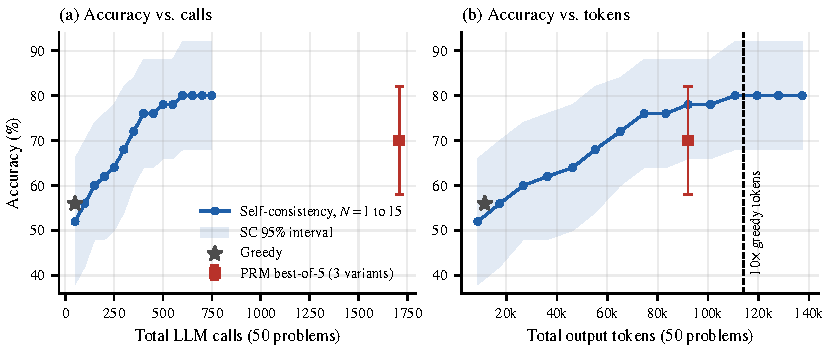
\includegraphics[width=\linewidth]{figures/scaling.pdf}
\caption{Accuracy against (a) total LLM calls and (b) total output tokens (generated plus judge). The three PRM variants coincide in cost and accuracy, and the bars are the interval of PRM min. The dashed line is ten times the greedy output tokens.}
\label{fig:scaling}
\end{figure}

PRM best-of-five reaches 70.0\% with every aggregation rule (Table~\ref{tab:main}), which is 14.0 pp above greedy decoding and 6.0 pp above SC-5. It wins 3 problems against SC-5 and loses none (Table~\ref{tab:paired}). Compute-matched SC-15 is more accurate than PRM search, 80.0\% against 70.0\%, with PRM winning 1 problem and losing 6. The product and step-penalty variants show the same pattern (4 wins and 1 loss against SC-5, and 1 and 2 wins against 6 and 7 losses against SC-15). Pool coverage explains part of the gap: a correct candidate exists among the five for 82\% of problems and among the fifteen for 92\%, so no selector over five candidates can pass 82\%. SC-15 also needs fewer LLM calls than PRM search (15 against 34.2 per problem) but emits more output tokens (2,746 against 1,841 per problem, where the PRM figure leaves out the much longer judge prompts; Figure~\ref{fig:scaling}).

\begin{table}[t]
\centering
\caption{Paired outcomes per problem for PRM min against each baseline. Diff is PRM minus baseline with a 95\% bootstrap interval. $p$ is an exact two-sided sign test on the problems where the two methods differ.}
\label{tab:paired}
\footnotesize
\begin{tabular}{lccccc}
\toprule
Baseline & PRM wins & Baseline wins & Both right / both wrong & Diff (pp) & $p$ \\
\midrule
Greedy & 10 & 3 & 25 / 12 & +14.0 [0.0, 28.0] & 0.092 \\
SC-5 & 3 & 0 & 32 / 15 & +6.0 [0.0, 14.0] & 0.250 \\
SC-15 & 1 & 6 & 34 / 9 & -10.0 [-22.0, 0.0] & 0.125 \\
\bottomrule
\end{tabular}
\end{table}

The intervals are wide. The interval for PRM minus SC-5 touches zero, as does the one against SC-15, and the sign tests give $p=0.25$ and $0.125$. We therefore treat the direction as the finding (PRM above SC-5 and below SC-15) and the size of the gaps as uncertain. Voting itself has a clearer effect: SC accuracy rises from 52.0\% at $N=1$ to 80.0\% at $N=12$ and then stays flat.

\section{Path Score Aggregation Ablation}
\begin{table}[t]
\centering
\caption{Aggregation ablation on the shared pool. Tie rate is the share of problems where more than one candidate reaches the maximum score. The last row is the optional probability variant.}
\label{tab:ablation}
\footnotesize
\begin{tabular}{lccc}
\toprule
Rule & $\lambda$ & Accuracy (\%) & Tie rate (\%) \\
\midrule
Min & n/a & 70.0 & 86.0 \\
Product & n/a & 70.0 & 34.0 \\
Step penalty & 0.0 & 70.0 & 72.0 \\
Step penalty & 0.5 & 70.0 & 70.0 \\
Step penalty & 2.0 & 70.0 & 70.0 \\
Product of $p_t$ (bonus) & n/a & \textbf{76.0} & 0.0 \\
\bottomrule
\end{tabular}
\end{table}

All five discrete settings reach 70.0\% (Table~\ref{tab:ablation}), although their tie rates range from 34\% to 86\%. With binary scores the rules differ as follows. Min-pooling gives only $-1$ or $+1$, so every fully valid path ties. The product $0.99^{T-k}\,0.01^{k}$ behaves like min-pooling, because one invalid step multiplies the score by 0.01 and a path with an invalid step therefore ranks below every fully valid path. It differs only among paths with the same $k$, where it prefers shorter paths, which breaks many ties but makes length the tie-break. The step penalty equals $1-(2/T+\lambda)k$. At $\lambda=0$ it ranks by the invalid fraction $k/T$, and as $\lambda$ grows it ranks mostly by $k$, which is why $\lambda=0.5$ and $\lambda=2$ have the same tie rate. In practice the rules disagree only when they choose between surviving candidates with different answers. The selected answer differs among min, product, and step penalty on 9 problems, and the changes cancel (min against step penalty: 1 win and 1 loss). Accuracy comes from discarding paths with an invalid step, and the ranking of the survivors matters little here.

Under min-pooling the judge filters and the majority vote chooses among the survivors. A tie occurs in 43 of 50 problems, with 3.7 of the 5 candidates tied on average. In 24 of these the tied candidates share one answer, so the vote is not needed. In the other 19 they disagree and the vote is correct 8 times. Taking the lowest-index tied path would also give 70.0\% on this run, but a uniformly random tied path would give 67.3\% in expectation, so an explicit tie rule is needed to avoid reducing the search to one random sample. In 10 problems no candidate is fully valid, and min-pooling then reduces to a vote.

The probability variant reaches 76.0\% with no ties, 6 pp above the discrete rules (three problems, within noise). Mean $p(\mathrm{valid})$ is 0.97 on steps judged valid and 0.09 on steps judged invalid (Figure~\ref{fig:judge}a), so the logits separate the two verdicts well, and the continuous score can prefer a confidently valid path over a barely valid one.

\section{Failure Modes and Judge Error Analysis}
\subsection{Judge Audit}
We labeled 40 judged steps by hand with the same local-validity rule given to the judge: 20 steps judged invalid and 20 judged valid, drawn at random within each group (seed 5326) from 29 problems. Table~\ref{tab:audit} gives the confusion matrix with invalid as the positive class. Precision is 45\% (9 of 20, Wilson 95\% interval [26, 66]) and recall is 82\% (9 of 11).

\begin{table}[t]
\centering
\caption{Judge audit of 40 steps against hand labels (invalid is positive).}
\label{tab:audit}
\footnotesize
\begin{tabular}{lccc}
\toprule
 & Human: invalid & Human: valid & Total \\
\midrule
Judge: invalid & TP = 9 & FP = 11 & 20 \\
Judge: valid & FN = 2 & TN = 18 & 20 \\
\bottomrule
\end{tabular}
\end{table}

More than half of the invalid verdicts are false alarms. Of the 11 false positives, three are plan-style steps with nothing to check (``Calculate the money left''), two are correct arithmetic or algebra that the judge evaluated wrongly, two penalize consistency with an earlier wrong step (a violation of local validity), and four are ambiguous. Both false negatives are conceptual and not arithmetic: one omits a cost, and the other defines profit as a final value. The two groups were sampled evenly, but the full run has only 348 invalid steps against 1,111 valid ones, so precision is a fair estimate while recall is optimistic. Reweighting the false-negative rate (2 of 20, Wilson [3, 30]\%) to all valid steps gives a recall near 58\% (plausible range 32 to 83\%). Over the whole run the judge flags 23.9\% of 1,459 steps. Paths with no flagged step are correct 77.2\% of the time (136 paths), and accuracy falls with the number of flagged steps (Figure~\ref{fig:judge}b), so the signal is real even though precision is low.

\begin{figure}[t]
\centering
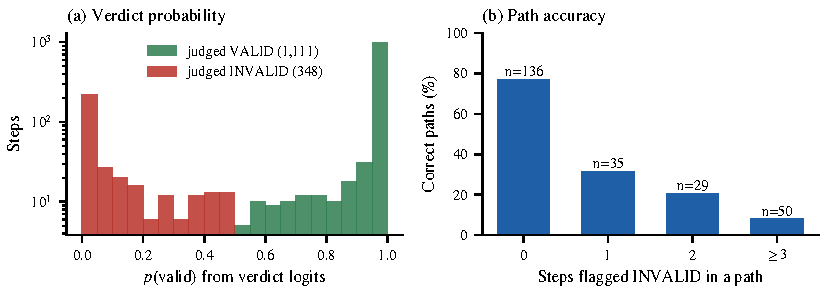
\includegraphics[width=\linewidth]{figures/judge.pdf}
\caption{(a) Verdict probability of the judge for steps judged valid and invalid (log scale). (b) Share of correct paths by the number of steps the judge flagged as invalid.}
\label{fig:judge}
\end{figure}

\subsection{Failure Cases}
\paragraph{Judge false positive.} In problem 03 (a house bought for \$80,000, \$50,000 of repairs, value up 150\%, answer 70,000), candidate 3 writes ``Subtract the original price from the new value to find the profit.'' The judge answers valid, with the rationale that the subtraction ``correctly calculates the profit'', but profit must subtract the price and the repairs, and the path returns 90,000. The judge accepts the generic form ``profit equals value minus price'' without tracking which costs the problem includes. It did flag two earlier steps of the same path.

\paragraph{Judge false negative.} In problem 31 (ages in the ratio 7:11, total 162), candidate 3 writes $A=(11/7)D$ after $D/A=7/11$. This is correct, but the judge answers invalid and argues that the ratio does not imply it. Without a written derivation, a 4-bit 7B model mishandles a one-line rearrangement, and because the rationale follows the verdict it justifies the decision and does not check it.

\paragraph{Shared flawed premise.} In problem 49 (a 4-foot wire cut into 6-inch pieces, answer 8), four of five candidates answer 24, and the judge marks every step of every path valid. The steps are plan-style (``Convert the length'', ``Divide the converted length'') and contain no numbers. The wrong arithmetic appears only in the final answer line, which the step judge never sees. Greedy decoding gives 8, but PRM and SC both choose 24, so voting amplifies the shared mistake. Over the whole run, 31 of 124 incorrect pool paths (25\%) pass every step, and four problems (08, 09, 13, 16) have no correct candidate among all fifteen.

\subsection{Stronger Judge than Generator}
A 7B judge can verify what a 1.5B generator writes. It detects arithmetic slips and misread quantities, and 77.2\% against 18.4\% accuracy for paths without and with a flagged step shows that this information is usable. It is a different model, so its errors are less likely to repeat the generator's, but it cannot see what a step omits and it over-flags correct work. If the 1.5B model verified its own paths, its errors would be correlated with the verdicts. The same misreading that produced a step would be accepted as valid. In problem 45 three of five candidates treat the cost of a pound of wax as a cost per candle, and the 7B judge rejects these paths, so PRM returns 20 where SC-5 returns $-160$. A 1.5B self-verifier would likely endorse them, remove few wrong candidates, and move PRM search toward plain sampling.

\section{Test-Time Compute Efficiency}
Greedy decoding generates 11,419 tokens over the 50 problems, so ten times that is 114,190 tokens. We count generated and judge output tokens against this budget (Table~\ref{tab:budget}). PRM search spends 92,056 tokens (80.6\% of the budget), but SC with $N=10$ spends 92,075 tokens for 78.0\%, and $N=12$ reaches 80.0\% at 97.0\% of the budget. Self-consistency is therefore the better use of a fixed output-token budget, by about 8 to 10 pp at equal cost.

\begin{table}[t]
\centering
\caption{Output tokens and accuracy against the budget of 114,190 tokens (10$\times$ greedy). PRM tokens are 46,349 generated plus 45,707 judge tokens.}
\label{tab:budget}
\footnotesize
\begin{tabular}{lccc}
\toprule
Method & Output tokens & Share of budget (\%) & Accuracy (\%) \\
\midrule
Greedy & 11,419 & 10.0 & 56.0 \\
SC-5 & 46,349 & 40.6 & 64.0 \\
PRM best-of-5 & 92,056 & 80.6 & 70.0 \\
SC, $N=10$ & 92,075 & 80.6 & 78.0 \\
SC, $N=12$ & 110,719 & 97.0 & 80.0 \\
SC-15 & 137,321 & 120.3 & 80.0 \\
\bottomrule
\end{tabular}
\end{table}

The costs of the two models are asymmetric. PRM search makes 1,459 judge calls for 250 generation calls (5.8 judge calls per path), so it uses 6.8 times the calls of SC-5. A judge call emits 31 tokens on average but reads 405 prompt tokens, while a generation call emits 185 tokens. Output-token counting therefore understates the cost of the judge, whose 591,199 prompt tokens are not counted, and wall-clock time agrees: PRM takes 3,875 s against 1,678 s for SC-15. Under a fixed budget we would spend the compute on self-consistency with a large $N$. This conclusion is limited by the 50-problem noise and by the quality of the prompted verifier.

\section{Reproducibility and Limitations}
Experiments ran on a Kaggle session with two Tesla T4 GPUs (14.6 GB each): the generator in FP16 on one and the judge in NF4 on the other, with generation and judging overlapped in two threads. Peak memory was not logged. The weights take about 3.1 GB (generator) and 5.5 GB (judge), and an earlier attempt with uncapped judge batches ran out of memory on the 14.6 GB judge GPU. The total wall-clock time was 3,138 s (52 min). Software versions are Python 3.13.16, PyTorch 2.11.0, transformers 5.20.2, accelerate 1.15.0, bitsandbytes 0.50.2, and NumPy 2.1.3. Each problem is seeded with $5326+\text{index}$, bootstrap resampling uses seed 5326, and per-problem checkpoints allow an interrupted run to resume. Judge prompts are therefore batched in groups of at most four with left padding, which can change results slightly through numerical differences from unbatched decoding. Prompts, parsers, and all artifacts are in the repository.

A prompted verifier is a weaker stand-in for a value function or a PRM trained on human step labels such as PRM800K \citep{lightman2023verify}. Such a model learns from labeled steps on the generator's own distribution to predict whether a prefix leads to a correct answer. The prompted judge has four limits here. First, it has no training signal for step correctness, and its 45\% precision reflects instruction following and not calibrated error detection. Second, it writes the verdict before the rationale, so it cannot compute the arithmetic it judges, which explains its errors on correct algebra and arithmetic. Third, local validity checks a step only against its prefix and does not estimate whether the path will succeed, so plan-style or incomplete paths pass. Fourth, quantization, prompt sensitivity, and binary outputs add noise that a calibrated scalar head would avoid, although the probability variant shows that raw logits already help. Further limits are the single seed, the 50-problem benchmark, and a hand audit of only 40 steps from one labeler.

\section{Conclusion}
A prompted step verifier scored 6 pp above five-sample self-consistency and 14 pp above greedy decoding, but fifteen samples with a plain vote scored 10 pp higher still, with fewer calls. With 50 problems, none of these gaps is established. The aggregation rule had no measurable effect, because the judge acts mainly as a filter. Its precision for invalid steps is 45\%, and a quarter of incorrect paths pass every step, so it detects errors that appear in a step and misses errors that do not. Under a fixed output-token budget, self-consistency is the better choice. A continuous verdict probability reached 76.0\% with no ties and is the most promising extension, but with 50 problems its advantage is not established.

\small
\begin{thebibliography}{10}
\bibitem[Brown et~al.(2024)]{brown2024monkeys}
Bradley Brown, Jordan Juravsky, Ryan Ehrlich, et~al. Large language monkeys: Scaling inference compute with repeated sampling. \emph{arXiv:2407.21787}, 2024.
\bibitem[Cobbe et~al.(2021)]{cobbe2021gsm8k}
Karl Cobbe, Vineet Kosaraju, Mohammad Bavarian, et~al. Training verifiers to solve math word problems. \emph{arXiv:2110.14168}, 2021.
\bibitem[Dettmers et~al.(2023)]{dettmers2023qlora}
Tim Dettmers, Artidoro Pagnoni, Ari Holtzman, and Luke Zettlemoyer. QLoRA: Efficient finetuning of quantized LLMs. In \emph{NeurIPS}, 2023.
\bibitem[Efron and Tibshirani(1993)]{efron1993bootstrap}
Bradley Efron and Robert Tibshirani. \emph{An Introduction to the Bootstrap}. Chapman and Hall, 1993.
\bibitem[Lightman et~al.(2023)]{lightman2023verify}
Hunter Lightman, Vineet Kosaraju, Yura Burda, et~al. Let's verify step by step. \emph{arXiv:2305.20050}, 2023.
\bibitem[Qwen Team(2024)]{qwen25}
Qwen Team. Qwen2.5 technical report. \emph{arXiv:2412.15115}, 2024.
\bibitem[Snell et~al.(2024)]{snell2024scaling}
Charlie Snell, Jaehoon Lee, Kelvin Xu, and Aviral Kumar. Scaling LLM test-time compute optimally can be more effective than scaling model parameters. \emph{arXiv:2408.03314}, 2024.
\bibitem[Wang et~al.(2023)]{wang2023selfconsistency}
Xuezhi Wang, Jason Wei, Dale Schuurmans, et~al. Self-consistency improves chain of thought reasoning in language models. In \emph{ICLR}, 2023.
\end{thebibliography}

\end{document}
